% kapitel3.tex
\externaldocument{02_grundlagen}
\externaldocument{04_implementierung}
\chapter{Fragestellung und Testmerkmale}
\label{chapter:fragestellung}

\section{Modellbildung}
\label{section:modellbildung}
Der im Rahmen dieder Abschlussarbeit vorgestellte Softwareprototyp basiert auf Vorarbeiten von Eidam et al. (\vgl \cite{Eidam2015,Eidam2016}) und dem aus dieser Arbeit entwickelten Softwareprototyp. Als eine alternative Kommunikationsmöglichkeit für Personen mit Sprach- und Bewegungseinschränkungen ermöglicht der Prototyp von Eidam et al. die Identifikation und Sonifikation von Bildobjekten auf austauschbaren Bildern mithilfe eines Eyetrackers. Diese vorliegende Arbeit erweitert diesen Ansatz um die Implementierung zweier unterschiedlicher Steuerungsmodelle für ein mobiles Robotersystem und um die Darstellung dynamischer Inhalte im Sinne eines Videobildes als \enquote{Live-Ansicht} im Vergleich zu statischen Inhalten.

Das in \acs{abb} \ref{fig:infotrans} skizzierte technisch unterstützte Kommunikationsverhalten zwischen Mensch und Umgebung,- kann nach Einführung der beteiligten Komponenten aus Kapitel \ref{chapter:grundlagen} zum erweiterten geplanten Interaktionsmodell für den Softwareprototyp ausgebaut werden.

\begin{figure}[ht]
\begin{minipage}[t]{\linewidth} 
      \centering 
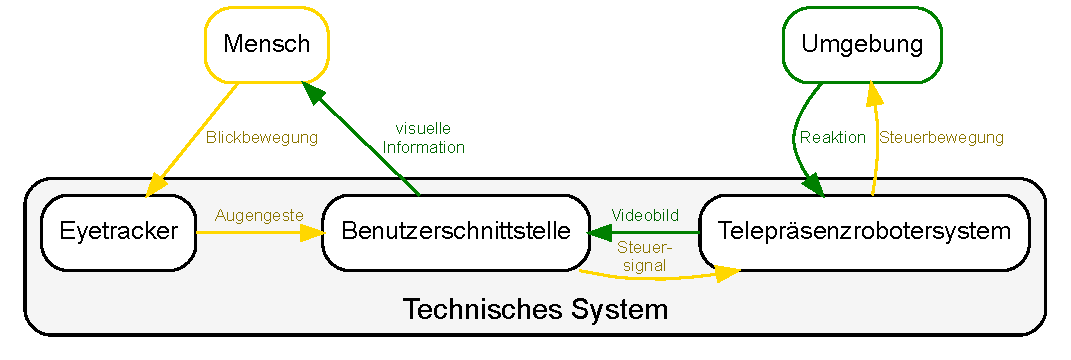
\includegraphics[width=\textwidth]{bilder/implementierung/komptrans.pdf}
   \end{minipage}% 
\caption{Die technisch unterstützte Kommunikation zwischen Mensch und Umgebung. Erweiterung der in \acs{abb}. \ref{fig:infotrans} auf Seite \pageref{fig:infotrans} grundsätzliche Ablauf der Kommunikation. Der Fokus liegt nun auf der Interaktion der einzelnen Komponenten des Systems.}
\label{fig:infotrans2}
\end{figure}

Die implementierten Steuerungsmodelle für das mobile Robotersystem sollen mittels eines selbst konzipierten Fragebogens untereinander verglichen und hinsichtlich der Machbarkeit, der Präzision, des Handlings, der Ermüdung und der Nutzung eines Panikschalters bewertet werden. 

Es folgt eine kurze einführende Beschreibung der beiden Steuerungsmodelle und Testmerkmale.

\section{Steuerungsmodell}
\label{section:steurungsmodell} 

\begin{comment}
\end{comment}
Nach Peters et al.~(2013) lassen sich haptische Eingabemechanismen nach mechanischen Gleichgewichtslagen aus der Physik einteilen, \vgl~\cite[S.118]{Peters2013}. Hiernach wird zwischen \textit{stabilen}, \textit{labilen} und \textit{indifferenten} Gleichgewichtslagen unterschieden, siehe \acs{abb}~\ref{fig:kugel} \cite{Peters2013}. Angewandt auf haptischen Eingabegeräte können sich in der Interaktion zwischen Eingabemechanismus und Benutzer die dynamischen Veränderungen des Mechanismus ebenfalls stabil, labil und indifferent verhalten.

\begin{figure}[ht]
\centering 
  \begin{minipage}[b]{0.8\linewidth} 
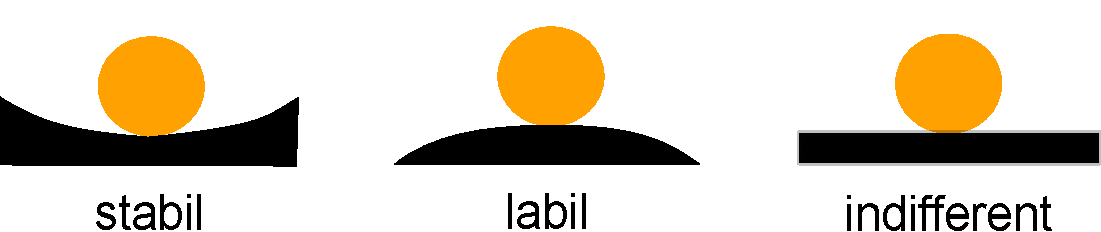
\includegraphics[width=\textwidth]{bilder/grundlagen/kugelang.pdf}
   \end{minipage}% 
   \hfill
   \caption{Mechanische Gleichgewichtslagen (\textit{stabil}, \textit{labil} und \textit{indifferent}) aus der Physik veranschaulicht am Beispiel einer Kugel \cite{Peters2013}. (Bild: angelehnt an \cite[S.118]{Peters2013})}\label{fig:kugel} 
\end{figure}

Allgemein können die bewährten Konzepte und Eigenschaften der haptischen Eingabegeräte auf grafische Steuerelemente übertragen werden. Auf dieser Grundlage wurde zur Steuerung eines mobilen Roboters, basierend auf Blickbewegungen, als erste Lösungsstrategie ein \textit{diskretes}~Steuermodell implementiert. Unter diesm Begriff des \textit{diskreten}~Steuermodells, wie er im Rahmen dieser vorliegenden Arbeit verwendet wird, ist eine Steuermethode zu verstehen, die nur während der Betätigung eines Steuerelements (siehe Kapitel~\ref{subsection:robotsteuerung}) ein vorgegebenes Bewegungssignal erzeugt. Damit handelt es sich, wie bei Peters et al.~(2013) beschrieben, um einen, in Analogie zu haptischen Eingabemechanismen, \textit{monostabilen} Mechanismus für den Informationstranfer \cite{Peters2013}. Das Steuerelement nimmt nur zwei endliche Wertzustände (\enquote{nicht betätigt = keine Bewegung}, \enquote{betätigt = festgelegte Bewegung}) an und wechselt jeweils in den Ausgangszustand (hier, in den Zustand \enquote{nicht betätigt}), falls keine Betätigung stattfindet. Die Betätigung des Steuerelements erfolgt durch eine Blickgeste (\acs{por} des Benutzers) innerhalb des angezeigten Bereiches eines Steuerelementes, (\vgl Kapitel~\ref{subsection:robotsteuerung}).

%Als erste Lösungsstrategie zur Steuerung eines mobilen Roboters, basierend auf Blickbewegungen, wurde ein \textit{diskretes} Steuermodell implementiert. Unter dem Begriff des \textit{diskreten} Steuermodells, wie es im Rahmen dieser vorliegenden Arbeit verwendet wird, ist eine Steuermethode zu verstehen, die nur während der Betätigung eines Steuerelements (siehe Kapitel \ref{subsection:robotsteuerung}) ein vorgegebenes Bewegungssignal erzeugt. Damit handelt es sich wie bei Peters et al. (2013) beschrieben um einen, in Analogie zu haptischen Eingabemechanismen, \textit{monostabilen} Mechanismus für den Informationstranfer \cite{Peters2013}. Das Steuerelement nimmt somit letztlich nur zwei endliche Wertzustände (\enquote{nicht betätigt = keine Bewegung}, \enquote{betätigt = festgelegte Bewegung}) an und wechselt jeweils in den Ausgangszustand. Die Betätigung des Steuerelements erfolgt durch eine Blickgeste, also den \acs{por} des Benutzers. 

Eine zweite Steuerungsform wurde als \textit{kontinuierliche} Steuermethode konzipiert. Diese Form des Informationsaustausches kann nach Peters et al.~(2013) in Analogie zu haptischen Eingabemechanismen als \textit{indifferenter} Mechanismus bezeichnet werden. Im Unterschied zu der \textit{diskreten} Steuermethode, erfolgt eine kontinuierliche Befehlserzeugung innerhalb eines definierten Wertebereichs (\enquote{keine Bewegung}-\enquote{maximale Bewegung}). Diese Werte werden durch jede Blickbewegung verändert. Diese Art der Steuerung ermöglicht eine differenzierte geschwindigkeits- und richtungsabhängige Befehlscodierung.  

\subsection{Diskretes Steuerungsmodell}
Das diskrete Steuerungsmodell stellt vier unterschiedliche Bewegungsrichtungen zur Verfügung. Hierbei werden zwei translationale Bewegungen in Vorwärts- und in Rückwärtsrichtung angeboten und jeweils die Drehung nach links und rechts. Somit ist diese Art der Steuerung vergleichbar mit einer Tastatursteuerung über die vier Richtungspfeiltasten\footnote{\url{https://de.wikipedia.org/wiki/Pfeiltaste} (letzter Aufruf: 18. Februar 2017)}. Die Bewegung findet jeweils während der Betätigung der Tasten statt. 

\subsection{Kontinuierliches Steuerungsmodell}
Wie eingangs erwähnt, stellt das kontinuierliche Steuermodell einen \textit{indifferenten} Eingabemechanismus bereit. Die Augen des Benutzers fungieren dabei als eine Art Steuerhebel (\enquote{Joystick})\footnote{\url{https://de.wikipedia.org/wiki/Joystick} (letzter Aufruf: 18. Februar 2017)}, wobei die beim Joystick gewohnte Rückkehr zur neutralen Ausgangsposition im vorliegenden Fall nicht passiv geschieht. Es ist leicht vorzustellen, dass jede Augenbewegung des Benutzers ein verändertes Bewegungssignal im Vergleich zum vorangegangen Befehl darstellt. Hierbei wurde zur Reduktion der Midas-Touch- Problematik eine Art \enquote{Neutralzone} im Zentrum des Blickfeldes durch einen farblich gekennzeichneten Bereich festgelegt, siehe Abschnitt~\ref{subsection:robotsteuerung}. Als Steuersignal werden die Blickbewegungen in Relation zur \enquote{Neutralstellung} im Sinne einer Translations- und Rotationsbewegung durch einen Algorithmus interpretiert. Translations- und Rotationsbewegungen können im Unterschied zur diskreten Steuerung in einer Bewegung simultan ausgeführt werden. Hierdurch soll ein erweiterter Bewegungsumfang im Vergleich zur diskreten Steuerungsmethode bereitgestellt werden.

\section{Testmerkmale der Steuerung}
\label{sect:testmerkmale}
Die beschriebenen Steuerungsmodelle werden anhand quantitativer und qualitativer Merkmale mithilfe des Fragebogens und der Parcoursbewältigungsaufgabe untersucht. Es folgt eine Auflistung der untersuchten Items. 
\begin{enumerate}
  \item Zur Klärung der Präzision und Machbarkeit der einzelnen Steuerungsmodelle wurde eine Parcoursaufgabe konzipiert und die Dauer, die zur Bewältigung benötigt wurde, quantifiziert.
  \item Die Frage der Präzision wurde mittels diochtomer Mehrfachantworten \bzgl unerwünschter Ausführungen während des gesamten Durchführungszeitraums erweitert. Hierfür wurden unerwünschte Ausführungen für folgende Merkmale erfragt: 
  \begin{enumerate}
  \item Blickbewegung
  \item Lidschluss
  \item Horizontale Augengeste
  \item Vertikale Augengeste
  \item Stoppmechanismus
  \item Steuerungskomandos
  \item Moduswechsel
  \item Sonstige
  \end{enumerate}
  Das Merkmal \enquote{Sonstige} ermöglicht die Angabe weiterer unerwünschter Ausführungen. 
  \item Die Frage der Ermüdung wurde mittels einer vierstufigen Ratingskala bewertet, dabei bedeuten: \enquote{1 = nicht ermüdend}, \enquote{2 = wenig ermüdend}, \enquote{3 = ermüdend}, \enquote{4 = sehr ermüdend}. 
  \item Die Frage der Einfachheit des Handlings wurde mittels einer Ordinalskala mit den Merkmalsausprägungen (\enquote{1 = sehr einfach}, \enquote{2 = einfach}, \enquote{3 = schwer}, \enquote{4 = sehr schwer}) erhoben.
 \item Die Frage der Nutzung des Panikschalters wurde mittels einer Ordinalskala mit den Merkmalsausprägungen (\enquote{1 = sehr einfach}, \enquote{2 = einfach}, \enquote{3 = schwer}, \enquote{4 = sehr schwer}) erhoben.
  \item Jedes Steuerungsmodell wurde einzeln mittels einer Ordinalskala mit Schulnoten als Merkmalsausprägungen (\enquote{1 = sehr gut}, \enquote{2 = gut}, \enquote{3 = befriedigend}, \enquote{4 = ausreichend}, \enquote{5 = mangelhaft}, \enquote{6 = ungenügend}) erhoben.
\end{enumerate}